\chapter{Servicios en móviles}\label{chap:7}
\section{Introducción al consumo de servicios desde móviles}
Esta sesión sirve de introducción al desarrollo de aplicaciones Android
utilizando Android Studio en Java.

En esta sesión se desarrolla una aplicación capaz de convertir euros
a dólares y viceversa.

Incialmente, se desarrolla un conversor simple que tiene el ratio de
conversión fijado en el código.
Posteriormente, se mejorará la aplicación utilizando una petición HTTP
que obtenga el ratio actualizado al momento.

\subsection{Converter simple}
Al crear el proyecto, seleccionamos el Android SDK Platform 33.

Posteriormente, creamos un dispositivo virtual que permita probar la
aplicación sin utilizar nuestro dispositivo físico.
Seleccionamos un Nexus 5X con Nougat (Android 7.0).

La interfaz de usuario consiste en dos campos de texto y dos botones.
Uno de los campos de texto contiene el valor en euros
y el otro la misma cantidad en dólares.
Al utilizar los botones se escribe en el otro campo de texto la cantidad
correspondiente en la moneda correspondiente.

Esto es, si se escribe el campo de texto de los euros
y se pulsa el botón de convertir a dólares,
se leerá la cantidad de euros del campo de texto de euros
y se escribirá la cantidad equivalente en dólares en el campo correspondiente.

La lógica de esta aplicación consiste en 3 funciones.

\begin{itemize}
    \item Función para convertir monedas en función de un ratio.
    \item Función para convertir de euros a dólares.
    \item Función para convertir de dólares a euros.
\end{itemize}

Por el momento se selecciona un valor fijo del ratio entre euros y dólares.

\subsection{Converter avanzado}
A continuación, se utilizará una API HTTP para obtener el ratio de euros a dólares.

Para acceder a esta API, se utilizará la libería Volley.
Para añadir Volley, utilizamos el manifiesto.

La API a utilizar (ExchangeRate) requiere que nos registremos y obtengamos un token
que nos permitirá realizar una cantidad fija de conversiones de forma gratuita.
Tras obtener dicho token, podemos introducirlo en la petición GET que realizamos con
Volley para obtener el ratio de conversión entre euros y dólares.

La petición de Volley no es instantánea, por lo que utilizamos una función de callback
que se ejecutará cuando llegue la respuesta a la petición de vuelta.
En esta función, extraemos de la respuesta el ratio de conversión y lo almacenamos
para poder utilizarlo en la función que convierte una moneda en otra.

Aquí se muestra un mensaje con el valor obtenido por la petición para el cambio de moneda:

\begin{minipage}{\linewidth}
	\centering
	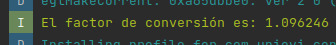
\includegraphics[width=\textwidth]{71/Conversion.jpg}
	\captionof{figure}{Ratio de EUR a USD}\label{fig:71/1}
\end{minipage}

A continuación, se muestra una captura de pantalla de la interfaz de usuario tras
haber realizado un cambio de euros a dólares:

\begin{minipage}{\linewidth}
	\centering
	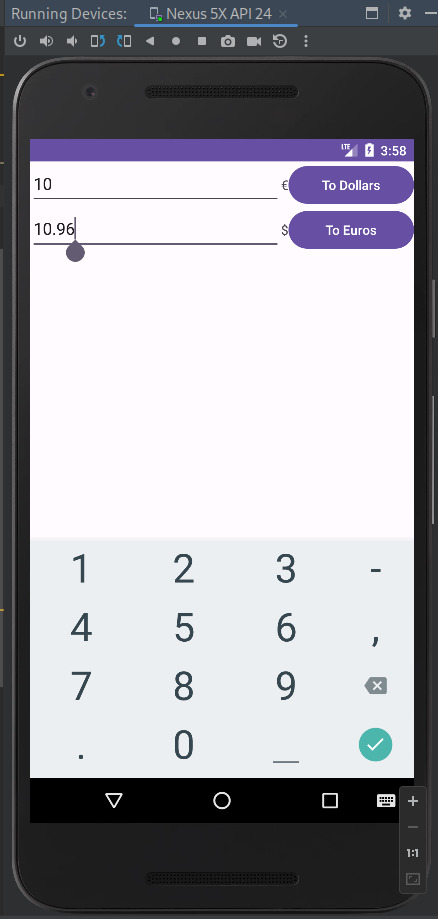
\includegraphics[width=0.4\textwidth]{71/App.jpg}
	\captionof{figure}{Aplicación}\label{fig:71/2}
\end{minipage}

\newpage{}
\section{Integración de servicios sobre móviles}\label{sec:7/2}
Durante esta sesión, se desarrolla una aplicación que pinta ``amigos'' en un mapa,
actualizando la posición de dichos amigos mediante llamadas al servicio API realizado
en la sesión 2.2 (Ver~\nameref{sec:2/2}).

\subsection{Pintar amigos en el mapa}
La primera parte de la sesión consiste en inicializar y configurar el proyecto y
ejecutar la aplicación de prueba sobre un emulador de Android. Puesto que se trata
de meramente seguir las instrucciones paso a paso del enunciado, no se incluyen
capturas de pantalla para evitar repetir lo mismo y alargar el documento.

El resultado de este apartado es el siguiente:

\begin{minipage}{\linewidth}
	\centering
	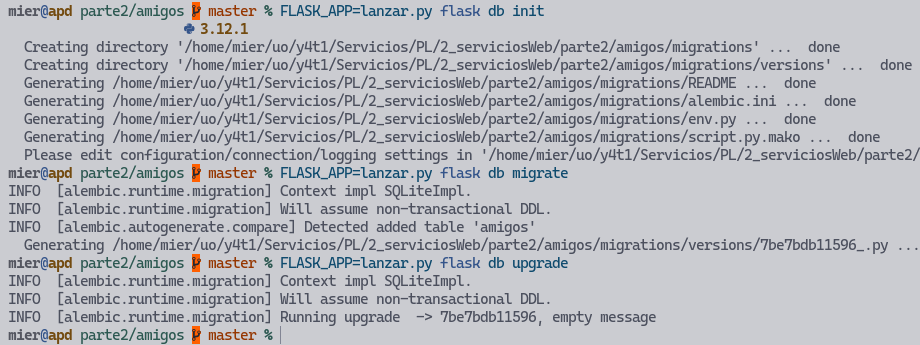
\includegraphics[width=0.3\textwidth]{72/1.png}
	\captionof{figure}{Aplicación base}\label{fig:72/1}
\end{minipage}

\subsection{Integración de servicios web}
En este apartado, se añade la funcionalidad de obtener la posición de los amigos. Para acceder
a la API, se utiliza la librería \Verb#Volley# que apunta hacia una URL generada por \Verb#ngrok#.

Tras seguir todas las instrucciones del enunciado, se consigue que la aplicación se conecte a la API,
obtenga la posición de los amigos y los pinte en el mapa cada cierto tiempo:

\begin{minipage}{\linewidth}
	\centering
	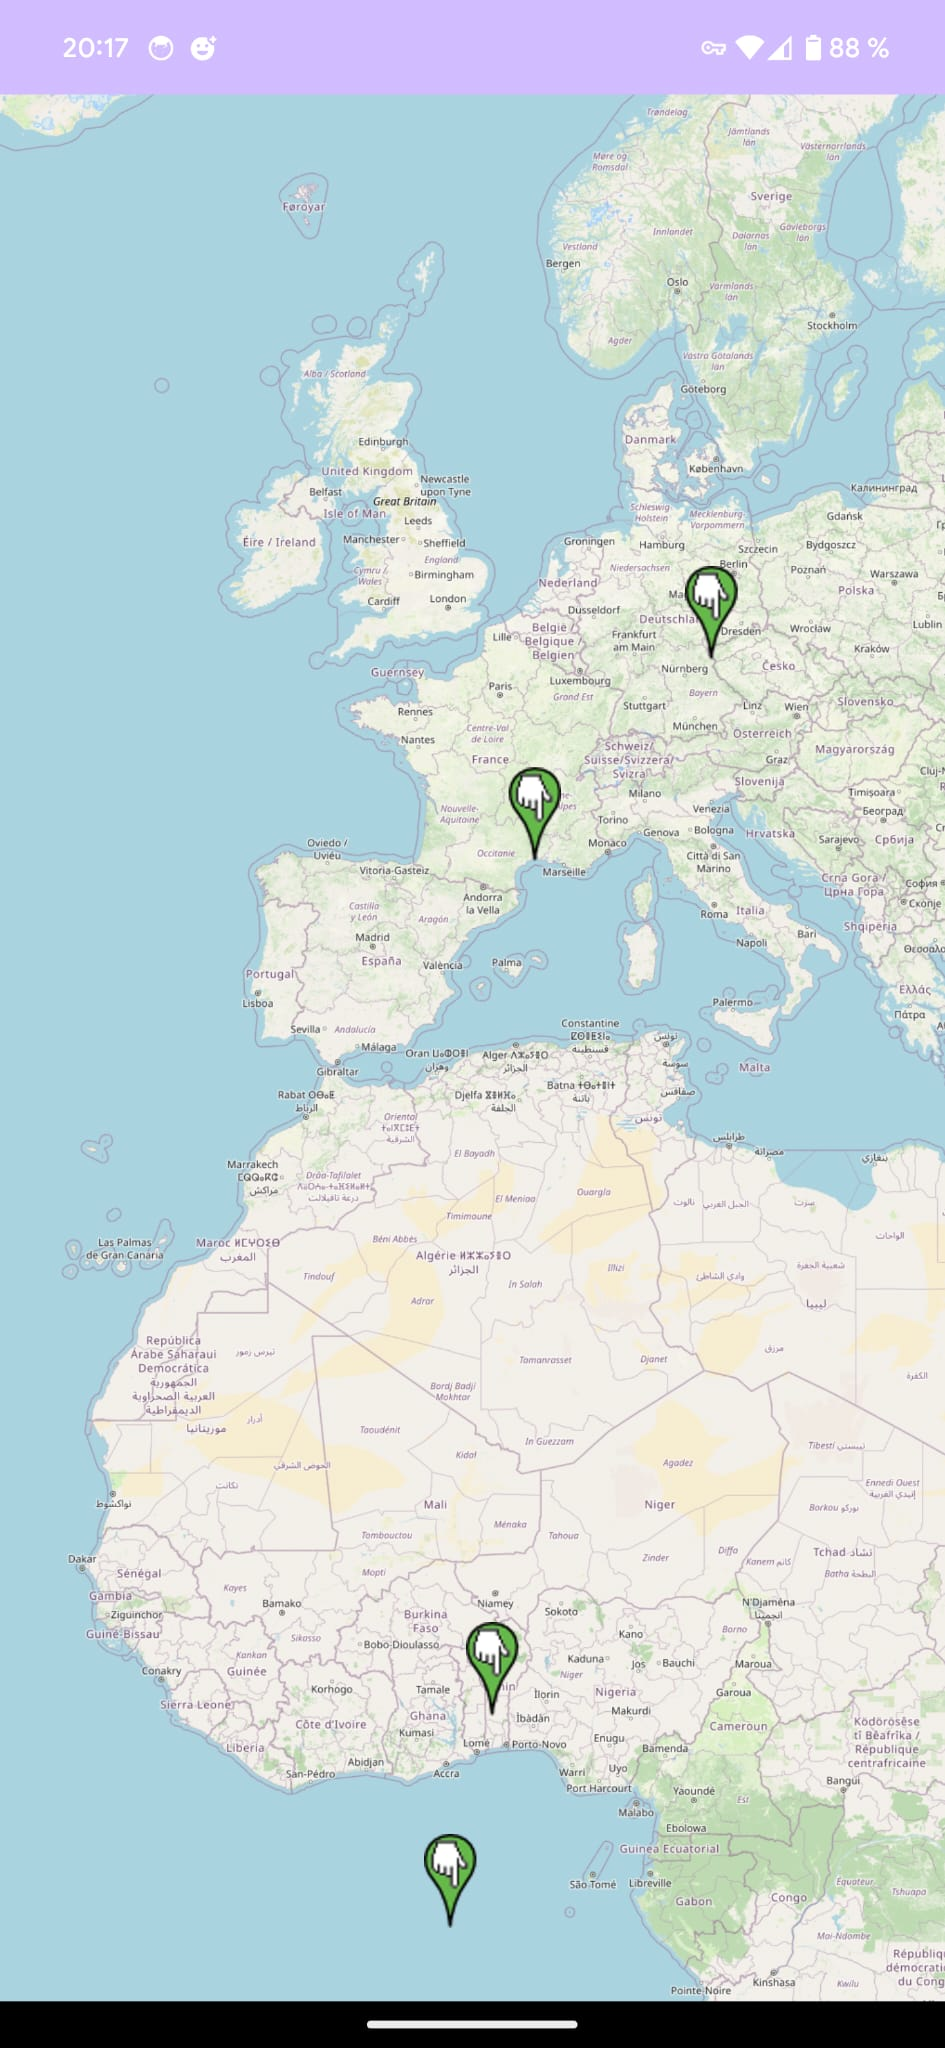
\includegraphics[width=0.3\textwidth]{72/2.png}
	\captionof{figure}{Aplicación con amigos pintados}\label{fig:72/2}
\end{minipage}

\begin{minipage}{\linewidth}
	\centering
	
\includegraphics[width=0.7\textwidth]{72/3.png}
	\captionof{figure}{Logcat de los amigos pintados}\label{fig:72/3}
\end{minipage}

\subsection{Actualización de la posición en función del GPS}
Esta parte de la práctica consiste en actualizar la posición de los amigos en función de la
posición del dispositivo móvil.

Lo primero de todo, se añade el permiso de acceso al GPS en el manifiesto de la aplicación.
Posteriormente, se añade la funcionalidad de obtener la posición del dispositivo móvil y
actualizar la posición de los amigos.

La única diferencia real con el enunciado de la práctica es que se evita pedir el nombre
al usuario por pantalla, ya que la interfaz que resulta no funciona correctamente en versiones
nuevas de Android (por causas desconocidas).

Procedemos a modificar la ubicación de uno de los usuarios utilizando el menú de Android Studio.
Inicialmente el usuario en cuestión se encontraba en DUMBO, NY, EEUU.
Tras el cambio de ubicación, el usuario se encontraba en Moscú, Russia.
Al esperar varios segundos, la interfaz de usuario del móvil emulado en Android Studio se modificó adecuadamente.

A continuación se muestran capturas de pantalla del cambio

\begin{minipage}{\linewidth}
	\centering
	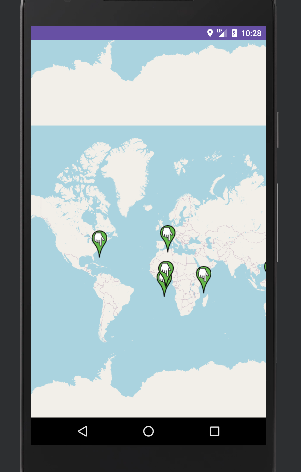
\includegraphics[width=0.7\textwidth]{72/app_dumbo.png}
	\captionof{figure}{Posición en DUMBO, NY}\label{fig:72/4}
\end{minipage}
\begin{minipage}{\linewidth}
	\centering
	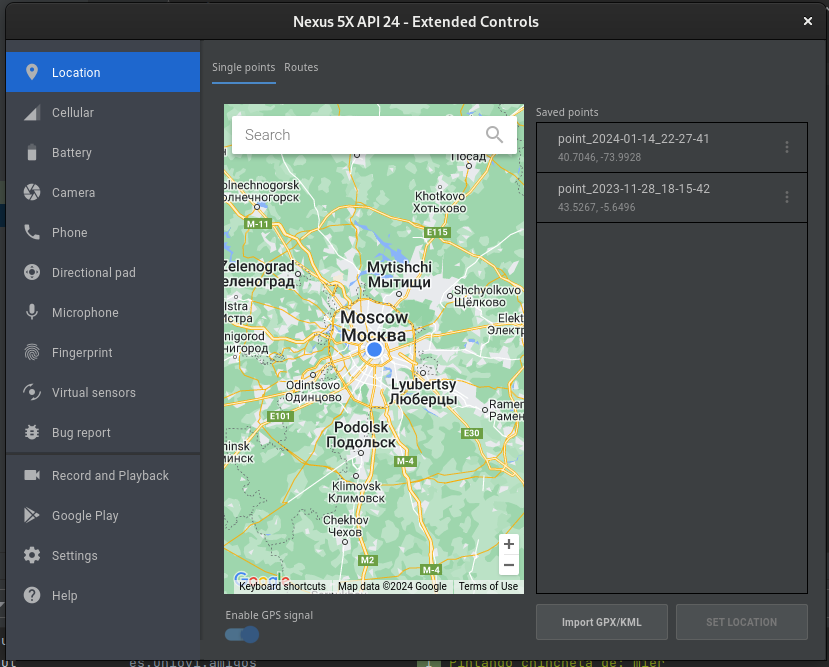
\includegraphics[width=0.7\textwidth]{72/app_switching_rus.png}
	\captionof{figure}{Cambiando la posición a Rusia}\label{fig:72/5}
\end{minipage}
\begin{minipage}{\linewidth}
	\centering
	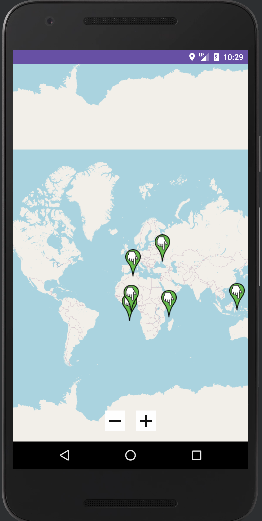
\includegraphics[width=0.7\textwidth]{72/app_rus.png}
	\captionof{figure}{Posición en Moscú, Rusia}\label{fig:72/6}
\end{minipage}

También se puede ver en la web

\begin{minipage}{\linewidth}
	\centering
	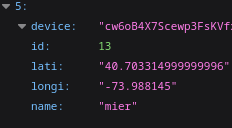
\includegraphics[width=0.7\textwidth]{72/json_dumbo}
	\captionof{figure}{Web: Posición en DUMBO, NY}\label{fig:72/7}
\end{minipage}
\begin{minipage}{\linewidth}
	\centering
	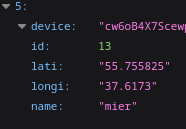
\includegraphics[width=0.7\textwidth]{72/json_rus}
	\captionof{figure}{Web: Posición en Moscú, Rusia}\label{fig:72/8}
\end{minipage}

\subsection{Servicios de notificaciones}

Tras realizar la preparación necesaria de Firebase, es necesario obtener el token en la aplicación Android.
Para ello, podemos filtrar el LogCat con 'FCM' para obtener dicho token.

En ese mismo filtro también se puede ver cómo la posición del amigo es modificada.

\begin{minipage}{\linewidth}
	\centering
	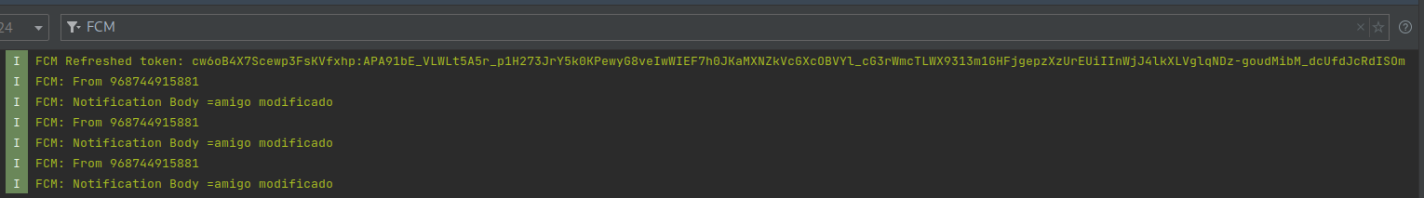
\includegraphics[width=0.7\textwidth]{72/FCM.png}
	\captionof{figure}{Token}\label{fig:72/9}
\end{minipage}

\section{Conclusiones}
Esta práctica es, sin duda, la más difícil de todas las realizadas. No por la dificultad de las
tareas a realizar, sino por la cantidad de potenciales problemas que surgen durante el desarrollo.
Uno de los más importantes, y el culpable de que la memoria de esta parte sea tan ``escueta'' es
un error introducido en alguna de las últimas versiones de Android Studio que hace imposible
ejecutar dispositivos virtuales debido a un fallo desconocido en la emulación.

\begin{minipage}{\linewidth}
	\centering
	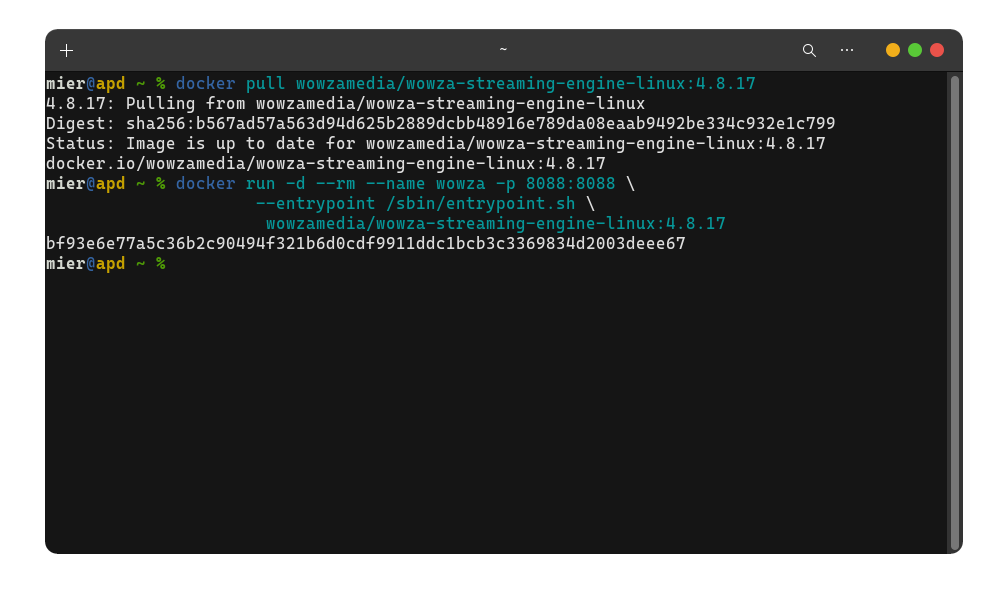
\includegraphics[width=0.9\textwidth]{72/4.png}
	\captionof{figure}{Error al ejecutar un dispositivo virtual}\label{fig:72/100000}
\end{minipage}

Otro error conocido es que no se logre la comunicación entre Firebase y la aplicación, pese a seguir
al pie de la letra todas las indicaciones del enunciado. Esto provoca que las chinchetas no se
actualicen o ni siquiera se lleguen a pintar en el mapa, pese a que esté todo ejecutándose correctamente.

Como introducción a la programación de aplicaciones móviles, esta práctica es muy interesante y
permite aprender mucho sobre el funcionamiento de las aplicaciones móviles y los problemas que
pueden surgir durante su desarrollo. Sin embargo, el hecho de tener que trabajar con todo el código en
un mismo fichero, juntado a todos los problemas surgidos durante el desarrollo, hacen que la experiencia no sea
nada satisfactoria.

Como nota personal, quiero resaltar que la explicación y longitud de la memoria de esta parte no refleja
el tiempo que se ha invertido. La mayor parte del tiempo se ha invertido en intentar solucionar los
problemas que han surgido durante el desarrollo, y no en el desarrollo en sí.

\begin{center}
	\begin{tabular}{|c|c|}
		\hline
		\textbf{Autor} & \textbf{Porcentaje} \\
		\hline
		\hline
		\authorOne & 70\% \\
		\authorTwo & 30\% \\
		\hline
	\end{tabular}
\end{center}
